
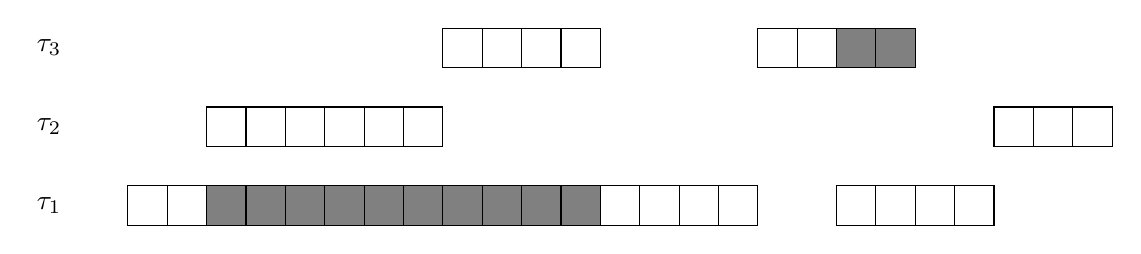
\begin{tikzpicture}
\node at(-1, 0.25) {$\tau_1$};
\node at(-1, 1.25) {$\tau_2$};
\node at(-1, 2.25) {$\tau_3$};
\draw[draw=black] (0, 0) rectangle ++(0.5,0.5) 
       node[pos=.5] {};
\draw[draw=black] (0.5, 0) rectangle ++(0.5,0.5) 
       node[pos=.5] {};
\draw[draw=black] (1, 1) rectangle ++(0.5,0.5) 
       node[pos=.5] {};
\draw[draw=black, fill=gray] (1, 0) rectangle ++(0.5,0.5) node[pos=.5, text=white] {};
\draw[draw=black] (1.5, 1) rectangle ++(0.5,0.5) 
       node[pos=.5] {};
\draw[draw=black, fill=gray] (1.5, 0) rectangle ++(0.5,0.5) node[pos=.5, text=white] {};
\draw[draw=black] (2, 1) rectangle ++(0.5,0.5) 
       node[pos=.5] {};
\draw[draw=black, fill=gray] (2, 0) rectangle ++(0.5,0.5) node[pos=.5, text=white] {};
\draw[draw=black] (2.5, 1) rectangle ++(0.5,0.5) 
       node[pos=.5] {};
\draw[draw=black, fill=gray] (2.5, 0) rectangle ++(0.5,0.5) node[pos=.5, text=white] {};
\draw[draw=black] (3, 1) rectangle ++(0.5,0.5) 
       node[pos=.5] {};
\draw[draw=black, fill=gray] (3, 0) rectangle ++(0.5,0.5) node[pos=.5, text=white] {};
\draw[draw=black] (3.5, 1) rectangle ++(0.5,0.5) 
       node[pos=.5] {};
\draw[draw=black, fill=gray] (3.5, 0) rectangle ++(0.5,0.5) node[pos=.5, text=white] {};
\draw[draw=black] (4, 2) rectangle ++(0.5,0.5) 
       node[pos=.5] {};
\draw[draw=black, fill=gray] (4, 0) rectangle ++(0.5,0.5) node[pos=.5, text=white] {};
\draw[draw=black] (4.5, 2) rectangle ++(0.5,0.5) 
       node[pos=.5] {};
\draw[draw=black, fill=gray] (4.5, 0) rectangle ++(0.5,0.5) node[pos=.5, text=white] {};
\draw[draw=black] (5, 2) rectangle ++(0.5,0.5) 
       node[pos=.5] {};
\draw[draw=black, fill=gray] (5, 0) rectangle ++(0.5,0.5) node[pos=.5, text=white] {};
\draw[draw=black] (5.5, 2) rectangle ++(0.5,0.5) 
       node[pos=.5] {};
\draw[draw=black, fill=gray] (5.5, 0) rectangle ++(0.5,0.5) node[pos=.5, text=white] {};
\draw[draw=black] (6, 0) rectangle ++(0.5,0.5) 
       node[pos=.5] {};
\draw[draw=black] (6.5, 0) rectangle ++(0.5,0.5) 
       node[pos=.5] {};
\draw[draw=black] (7, 0) rectangle ++(0.5,0.5) 
       node[pos=.5] {};
\draw[draw=black] (7.5, 0) rectangle ++(0.5,0.5) 
       node[pos=.5] {};
\draw[draw=black] (8, 2) rectangle ++(0.5,0.5) 
       node[pos=.5] {};
\draw[draw=black] (8.5, 2) rectangle ++(0.5,0.5) 
       node[pos=.5] {};
\draw[draw=black] (9, 0) rectangle ++(0.5,0.5) 
       node[pos=.5] {};
\draw[draw=black, fill=gray] (9, 2) rectangle ++(0.5,0.5) node[pos=.5, text=white] {};
\draw[draw=black] (9.5, 0) rectangle ++(0.5,0.5) 
       node[pos=.5] {};
\draw[draw=black, fill=gray] (9.5, 2) rectangle ++(0.5,0.5) node[pos=.5, text=white] {};
\draw[draw=black] (10, 0) rectangle ++(0.5,0.5) 
       node[pos=.5] {};
\draw[draw=black] (10.5, 0) rectangle ++(0.5,0.5) 
       node[pos=.5] {};
\draw[draw=black] (11, 1) rectangle ++(0.5,0.5) 
       node[pos=.5] {};
\draw[draw=black] (11.5, 1) rectangle ++(0.5,0.5) 
       node[pos=.5] {};
\draw[draw=black] (12, 1) rectangle ++(0.5,0.5) 
       node[pos=.5] {};
\end{tikzpicture}
